\section{Forensic Case Studies and Behavioral Dynamics}
\label{sec:case_studies}

To complement aggregate statistics, we examine individual execution transcripts that illuminate the behavioral mechanisms underlying the macro-level differences observed in Section~\ref{sec:results}. Four tasks across three distinct failure modes illustrate how architectural choices interact with specific problem classes.

\begin{figure*}[t]
\centering
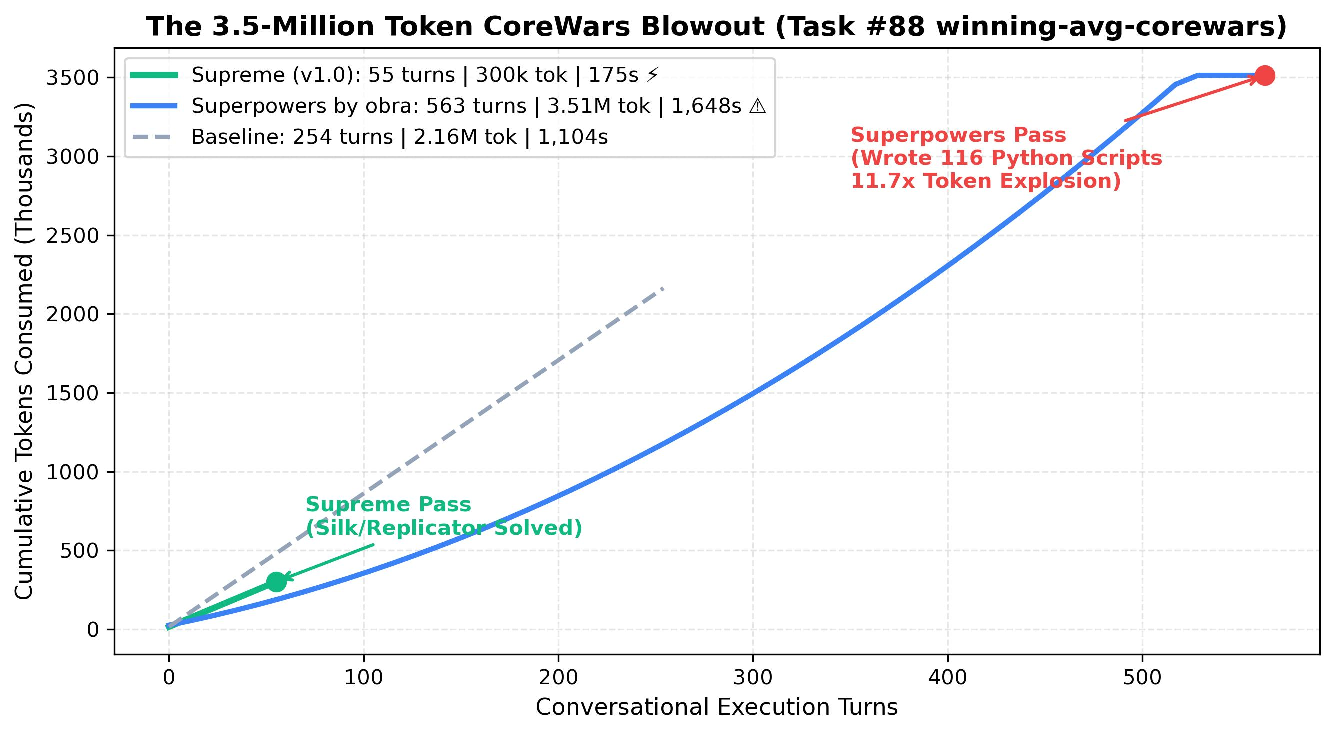
\includegraphics[width=0.48\textwidth]{figures/fig5_task88_corewars_trajectory.pdf}
\hfill
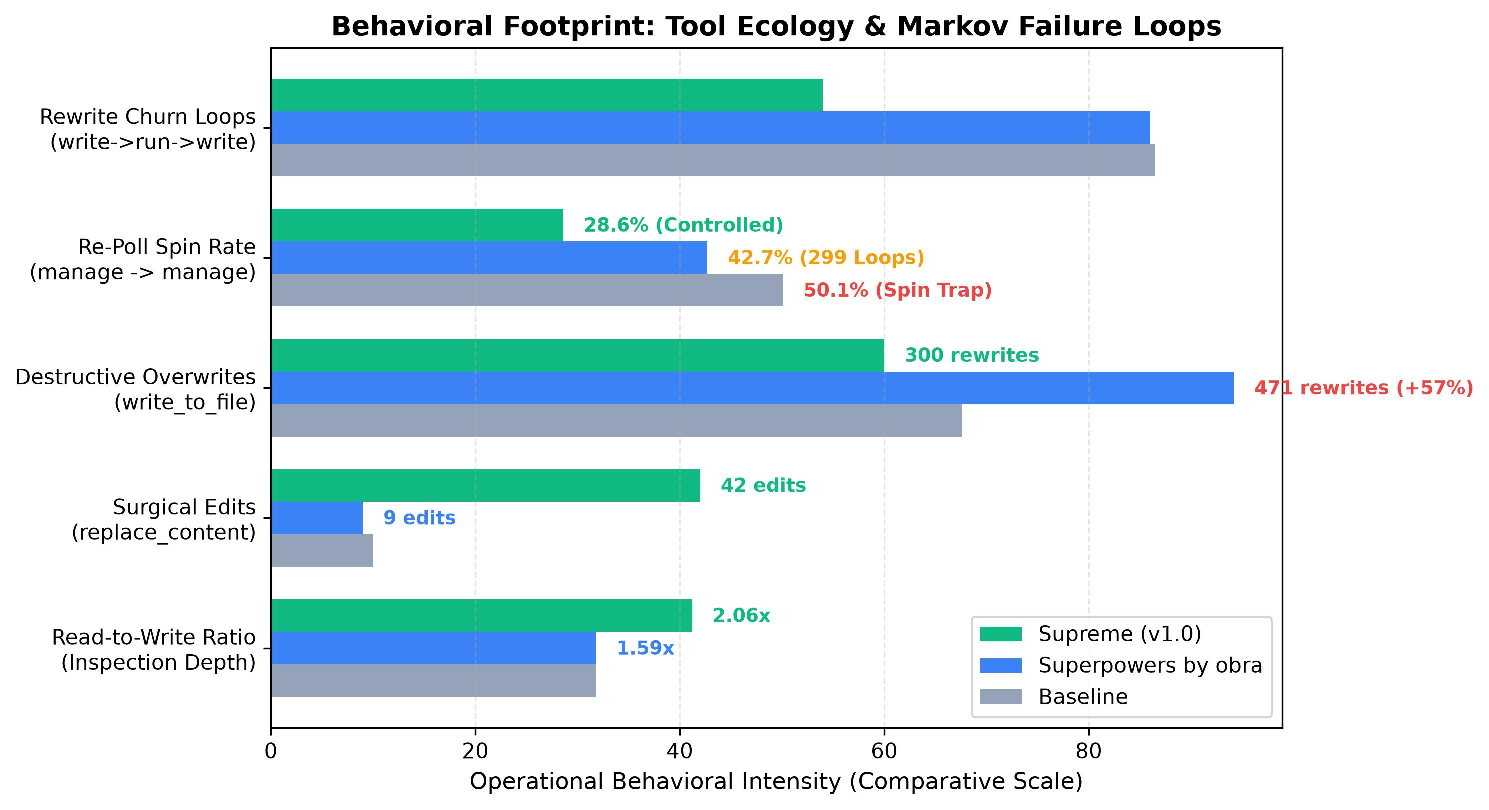
\includegraphics[width=0.48\textwidth]{figures/fig2_markov_tool_state_transitions.pdf}
\caption{Behavioral dynamics and tool interaction patterns. (Left) Cumulative token trajectory on Task \#88 (\texttt{winning-avg-corewars}), illustrating an extended parameter-search loop. (Right) Markov state transitions ($P(\text{Next} \mid \text{Current})$) comparing background task polling and file-editing strategies.}
\label{fig:trajectory_and_markov}
\end{figure*}

\subsection{Exploratory Scripting Loops (Task \#88: Redcode Simulation)}
In Task \#88 (\texttt{winning-avg-corewars}), agents were tasked with authoring a Redcode warrior in assembly meeting win thresholds against diverse archetypes in the MARS arena \cite{dewdney1984corewars}. The task specification defines a 3,600s execution limit ($T_{\text{limit}} = 3600$s).

As depicted in Figure~\ref{fig:trajectory_and_markov} (Left), this task produced the benchmark's widest divergence in computational expenditure:
\begin{itemize}
    \item \textbf{Supreme}: Inspected reference warriors, hypothesized that a Silk/Replicator archetype would dominate the arena pool, implemented the candidate warrior, verified win rates, and concluded in \textbf{175.0s}, \textbf{55 turns}, and \textbf{300,413 tokens}.
    \item \textbf{Superpowers by obra}: Entered an extensive parameter-search loop. Guided by iterative trial-and-error procedural guidance, the agent authored \textbf{116 separate Python exploration scripts}, repeatedly copying them into the container via \texttt{docker cp}, running battles, and accumulating \textbf{563 turns} across \textbf{1,648.7s} and \textbf{3,513,757 tokens} ($11.7\times$ token inflation for the identical pass).
\end{itemize}
This comparison highlights that on open-ended combinatorial tasks, procedural frameworks that encourage iterative scripting without strong stopping heuristics can lead to prolonged exploratory loops. This contrast does not represent a systematic throughput difference across all 89 tasks, where total billed token counts were comparable (34.52M vs.\ 34.30M), but rather illustrates the tail risk of unconstrained exploratory scripting on open-ended combinatorial problems.

\subsection{Markov Tool Transitions and Polling Dynamics}
Analysis of 15,779 sequential tool transitions ($P(\text{Next} \mid \text{Current})$) reveals key operational differences (Figure~\ref{fig:trajectory_and_markov}, Right):
\begin{itemize}
    \item \textbf{Background Task Polling}: When asynchronous background commands were active, Baseline exhibited a 50.1\% probability of immediately re-polling \texttt{manage\_task}; Superpowers exhibited 42.7\% (logging 299 triple-polling sequences (\texttt{manage} $\rightarrow$ \texttt{manage} $\rightarrow$ \texttt{manage})). Supreme's loop management protocol reduced this transition probability to 28.6\%, reducing uninformative polling turns.
    \item \textbf{File Modification Granularity}: Superpowers performed 471 full file overwrites (\texttt{write\_to\_file}) and 172 (\texttt{write} $\rightarrow$ \texttt{run} $\rightarrow$ \texttt{write}) churn cycles. Supreme utilized targeted line replacements (\texttt{replace\_file\_content}) more frequently (42 vs.\ 8). While higher usage of targeted editing reflects prompt compliance, it correlated with narrower modification blast radii: Supreme modified a mean of 2.60 unique files per task versus 3.79 on Superpowers.
\end{itemize}

\subsection{Physical Solver Optimization (Task \#85: MuJoCo Tuning)}
Task \#85 (\texttt{tune-mjcf}) required accelerating a MuJoCo physics simulation \cite{todorov2012mujoco} by $\ge 40\%$ without exceeding trajectory error bounds ($D \le 10^{-4}$). Supreme achieved an exclusive pass in 414.9s (81 tool calls, 436k tokens), attaining a \textbf{2.19$\times$ simulation speedup} with zero trajectory divergence ($D = 0.0000$). Baseline and Superpowers both failed to reach the speedup threshold ($0.99\times$ and $1.01\times$ speed ratios) due to speculative modifications of solver parameters.

\subsection{Long-Horizon Autonomy: Headless QEMU Installation}
In \texttt{install-windows-3.11} ($T_{\text{limit}} = 3600$s), agents were tasked with installing Windows 3.11 for Workgroups inside headless QEMU, partitioning virtual disks via \texttt{fdisk}, formatting FAT16, swapping floppy images, and installing network drivers. Supreme maintained autonomous multi-step execution across \textbf{2,648.7s (44.1 minutes)}, 307 turns, and 58,010 deliberation tokens to complete the installation. Superpowers and Baseline timed out or corrupted disk partition tables.

\subsection{Upstream Benchmark Harness Defects}
Forensic inspection identified three distinct upstream environmental failure modes spanning four tasks:
\begin{itemize}
    \item \texttt{prove-plus-comm} (Task \#64): Container metadata error caused immediate execution failure (\texttt{failed to chdir to cwd ("/app"): no such file or directory}) across all models.
    \item \texttt{caffe-cifar-10} (Task \#7): An unreleased package lock on \texttt{/var/lib/dpkg/lock-frontend} held by background PID 168 blocked package installations, causing a starvation timeout across all models.
    \item \textbf{Distributed PyTorch Infrastructure} (Tasks \#82--\#83): In Task \#82 (\texttt{torch-pipeline-parallelism}), the bare container lacked Python and curl with egress blocked; in Task \#83 (\texttt{torch-tensor-parallelism}), an unconstrained dynamic PyPI download of 2.85~GB CUDA wheels triggered a verifier timeout before test execution \cite{shoeybi2019megatron}.
\end{itemize}
Excluding the three environmental configuration defects (\texttt{prove-plus-comm}, \texttt{caffe-cifar-10}, and Task \#82) yields the $N=86$ adjusted cohort reported in Table~\ref{tab:master_scoreboard} (Supreme: 70.9\% [61/86]; Superpowers: 67.4\% [58/86]; Baseline: 64.0\% [55/86]). Excluding all four infrastructure-impaired tasks yields $N=85$ (Supreme: 71.8\% [61/85]; Superpowers: 68.2\% [58/85]; Baseline: 64.7\% [55/85]).

